\documentclass[tikz,border=12pt]{standalone}
\usepackage{helvet}
\renewcommand{\familydefault}{\sfdefault}
\usepackage{tikz}
\usetikzlibrary{positioning, fit, calc, shapes.geometric, arrows.meta}

\definecolor{emeraldpine}{HTML}{1A4D3E}
\definecolor{harvardcrimson}{HTML}{A51C30}
\definecolor{ethdarkblue}{HTML}{1F407A}
\definecolor{ethpetrol}{HTML}{007A87}
\definecolor{ethbronze}{HTML}{B87333}
\definecolor{ink}{HTML}{1A202C}
\definecolor{softink}{HTML}{4A5568}
\definecolor{paleink}{HTML}{A0AEC0}
\definecolor{cardbg}{HTML}{F8FAFC}
\definecolor{shadecolor}{HTML}{F4F6F9}

\begin{document}
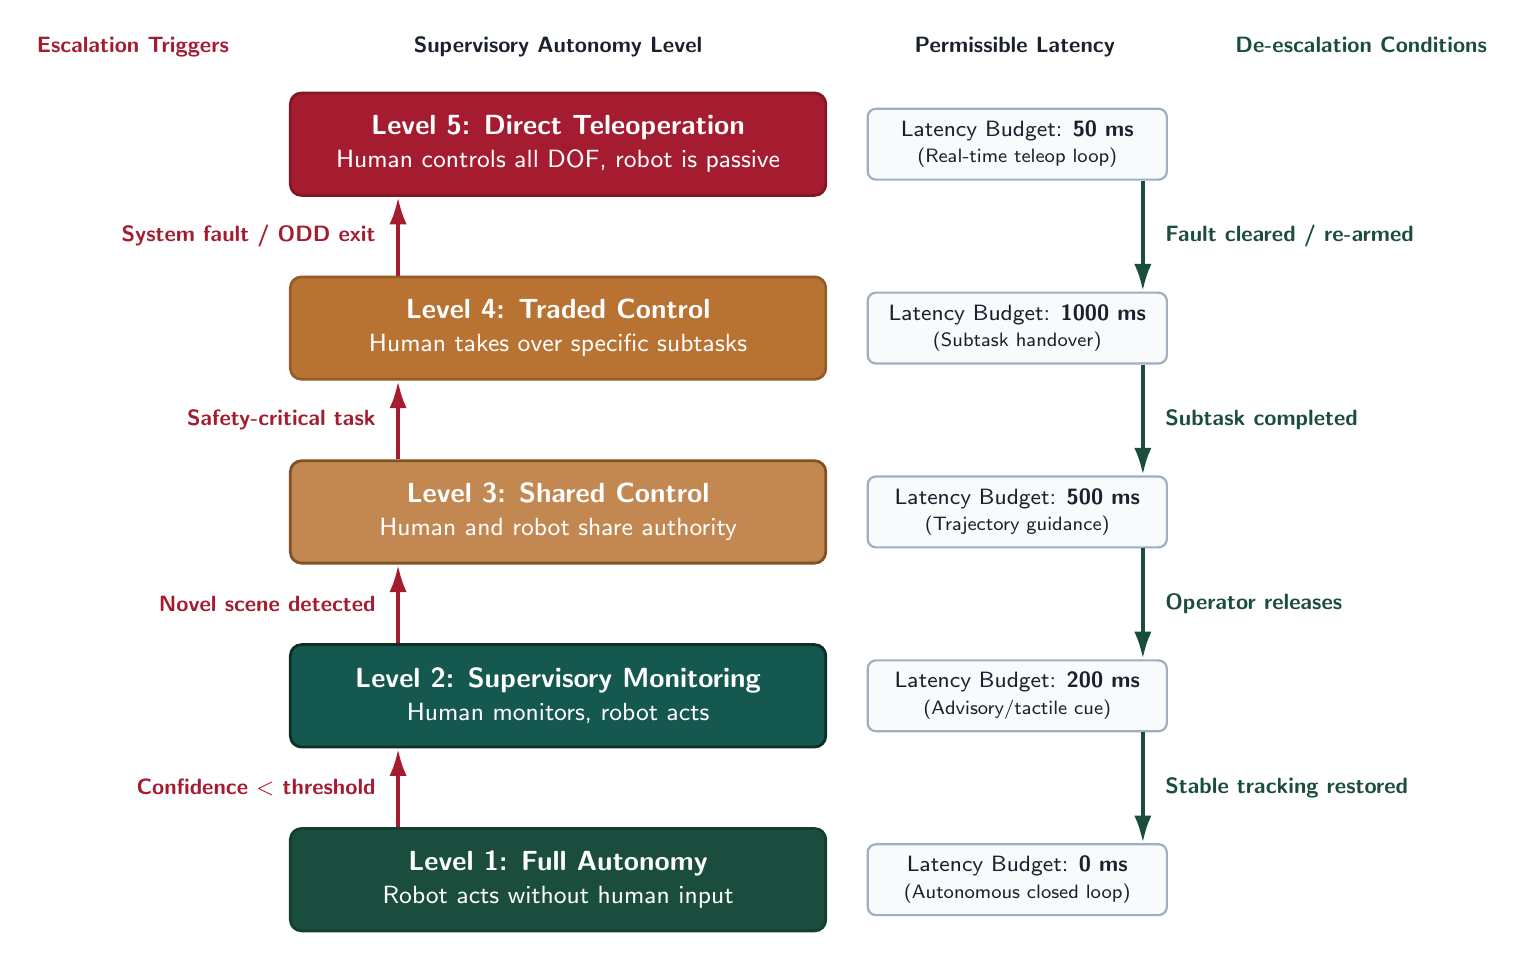
\begin{tikzpicture}[
    font=\sffamily,
    rung/.style={
        rectangle, 
        rounded corners=4pt, 
        minimum width=6.8cm, 
        minimum height=1.3cm, 
        align=center,
        text=white,
        font=\bfseries\normalsize,
        line width=1pt
    },
    latency/.style={
        rectangle,
        rounded corners=3pt,
        fill=cardbg,
        text=ink,
        font=\footnotesize,
        inner sep=4pt,
        draw=paleink,
        line width=0.8pt,
        minimum width=3.8cm,
        minimum height=0.9cm,
        align=center
    },
    escalate/.style={
        -{Latex[length=3.5mm, width=2.2mm]},
        line width=1.6pt,
        draw=harvardcrimson,
    },
    deescalate/.style={
        -{Latex[length=3.5mm, width=2.2mm]},
        line width=1.6pt,
        draw=emeraldpine,
    },
    triggerlabel/.style={
        font=\footnotesize\bfseries,
        text=harvardcrimson,
        align=right
    },
    release/.style={
        font=\footnotesize\bfseries,
        text=emeraldpine,
        align=left
    },
    colheader/.style={
        font=\sffamily\bfseries\footnotesize,
        align=center
    }
]

% Rungs
\node[rung, fill=emeraldpine, draw=emeraldpine!80!black] (l1) at (0, 0) {Level 1: Full Autonomy\\ \normalfont\small Robot acts without human input};
\node[rung, fill=emeraldpine!75!ethpetrol, draw=emeraldpine!60!black, above=1.0cm of l1] (l2) {Level 2: Supervisory Monitoring\\ \normalfont\small Human monitors, robot acts};
\node[rung, fill=ethbronze!85, draw=ethbronze!70!black, text=white, above=1.0cm of l2] (l3) {Level 3: Shared Control\\ \normalfont\small Human and robot share authority};
\node[rung, fill=ethbronze, draw=ethbronze!80!black, text=white, above=1.0cm of l3] (l4) {Level 4: Traded Control\\ \normalfont\small Human takes over specific subtasks};
\node[rung, fill=harvardcrimson, draw=harvardcrimson!80!black, above=1.0cm of l4] (l5) {Level 5: Direct Teleoperation\\ \normalfont\small Human controls all DOF, robot is passive};

% Latency Badges
\node[latency, right=0.5cm of l1.east] (lat1) {Latency Budget: \textbf{0 ms}\\\scriptsize (Autonomous closed loop)};
\node[latency, right=0.5cm of l2.east] (lat2) {Latency Budget: \textbf{200 ms}\\\scriptsize (Advisory/tactile cue)};
\node[latency, right=0.5cm of l3.east] (lat3) {Latency Budget: \textbf{500 ms}\\\scriptsize (Trajectory guidance)};
\node[latency, right=0.5cm of l4.east] (lat4) {Latency Budget: \textbf{1000 ms}\\\scriptsize (Subtask handover)};
\node[latency, right=0.5cm of l5.east] (lat5) {Latency Budget: \textbf{50 ms}\\\scriptsize (Real-time teleop loop)};

% Column Headers (aligned horizontally)
\coordinate (hdrY) at ([yshift=0.5cm]l5.north);
\node[colheader, text=harvardcrimson, anchor=base] at (-5.4, 0 |- hdrY) {Escalation Triggers};
\node[colheader, text=ink, anchor=base] at (0, 0 |- hdrY) {Supervisory Autonomy Level};
\node[colheader, text=ink, anchor=base] at (5.8, 0 |- hdrY) {Permissible Latency};
\node[colheader, text=emeraldpine, anchor=base] at (10.2, 0 |- hdrY) {De-escalation Conditions};

% Escalation Arrows (Left) - consistent vertical geometry
\draw[escalate] ([xshift=-0.6cm]l1.155) -- ([xshift=-0.6cm]l2.205) 
    node[midway, left=4pt, triggerlabel] {Confidence $<$ threshold};
\draw[escalate] ([xshift=-0.6cm]l2.155) -- ([xshift=-0.6cm]l3.205) 
    node[midway, left=4pt, triggerlabel] {Novel scene detected};
\draw[escalate] ([xshift=-0.6cm]l3.155) -- ([xshift=-0.6cm]l4.205) 
    node[midway, left=4pt, triggerlabel] {Safety-critical task};
\draw[escalate] ([xshift=-0.6cm]l4.155) -- ([xshift=-0.6cm]l5.205) 
    node[midway, left=4pt, triggerlabel] {System fault / ODD exit};

% De-escalation Arrows (Right) - matching vertical geometry
\draw[deescalate] ([xshift=0.6cm]lat5.335) -- ([xshift=0.6cm]lat4.25) 
    node[midway, right=4pt, release] {Fault cleared / re-armed};
\draw[deescalate] ([xshift=0.6cm]lat4.335) -- ([xshift=0.6cm]lat3.25) 
    node[midway, right=4pt, release] {Subtask completed};
\draw[deescalate] ([xshift=0.6cm]lat3.335) -- ([xshift=0.6cm]lat2.25) 
    node[midway, right=4pt, release] {Operator releases};
\draw[deescalate] ([xshift=0.6cm]lat2.335) -- ([xshift=0.6cm]lat1.25) 
    node[midway, right=4pt, release] {Stable tracking restored};

\end{tikzpicture}
\end{document}
